\documentclass[11pt]{preprint}

\setlength{\topmargin}{0mm} \setlength{\oddsidemargin}{0mm}
\setlength{\textwidth}{160mm} \setlength{\textheight}{215mm}

\usepackage{amssymb,amsmath,amscd,amsthm}
\usepackage{tikz}

\def\enumb{\begin{enumerate}}
\def\enume{\end{enumerate}}
\def\itemb{\begin{itemize}}
\def\iteme{\end{itemize}}
\def\integers{\mathbb{Z}}



\newtheorem{proposition}{Proposition}
\newtheorem{theorem}{Theorem}

\title{Discrete Mathematics, 2016 Fall - Worksheet 8}
\author{Instructor: Zsolt Pajor-Gyulai, CIMS}
\date{October 2, 2016}



\begin{document}

\maketitle

In all of the above problems explain your answer in full English sentences.

\enumb

\item Evaluate the following without doing any writing or arithmetic.
\enumb
\item $\binom{9}{0}$
\item $\binom{9}{1}$
\item $\binom{9}{8}$
\item $\binom{9}{6}-\binom{9}{3}$
\item $\binom{0}{0}$
\item $\binom{0}{2}$
\enume

\item Write out all $3$-element subsets of $\{1,2,3,4,5,6\}$ to verify that $\binom{6}{3}=20$.
\item Twenty people attend a party. If everyone shakes everyone else's hand exactly once, how many handshakes take place?
\item Prove that 
\[
2^n=\sum_{k=0}^{n}\binom{n}{k}.
\]
One easy way is to substitute $x=y=1$ into the binomial theorem. However, please give a combinatorial proof.

\item 
\enumb
\item Use the binomial theorem to prove
\[
\binom{n}{0}-\binom{n}{1}+\binom{n}{2}-\binom{n}{3}+\dots\pm\binom{n}{n}=0
\]
\item Move all the negative terms over to the right hand side to give
\[
\binom{n}{0}+\binom{n}{2}+\binom{n}{4}+\dots=\binom{n}{1}+\binom{n}{3}+\binom{n}{5}+\dots
\]
Give a combinatorial interpretation of this identity.
\enume

\item Consider the following formula. Give two different proofs one using the factorial formula, the other being a combinatorial proof.
\[
\binom{2n+2}{n+1}=\binom{2n}{n+1}+2\binom{2n}{n}+\binom{2n}{n-1}
\]


\item What is the coefficient of $x^3$ in $(2x-3)^6$?
\item (Counting lattice paths) Consider a grid such as the one shown in the figure. We want to count the number of paths from the lower left corner to the upper right corner in which each step of the path either goes one unit to the right or one unit upwards (e.g. the bold one on the picture). How many such path are there? (If you are stuck, you can look at p97 of the textbook.)
\begin{figure}[h]
\centering
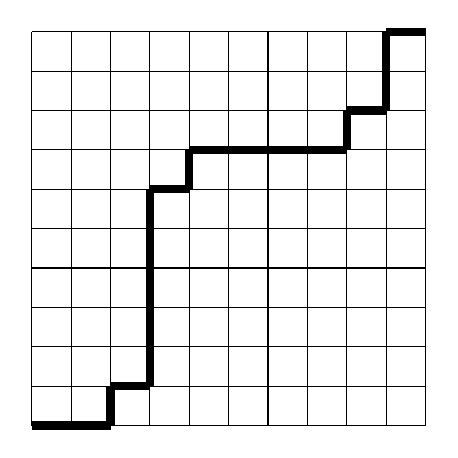
\begin{tikzpicture}[scale=0.5]
\foreach \i in {0,1,2,3,4,5,6,7,8,9,10}
	{
		\draw (\i,0) -- (\i,10);
	}
	
\foreach \i in {0,1,2,3,4,5,6,7,8,9,10}
	{
		\draw (0,\i) -- (10,\i);
	}
	
\draw[line width=3pt] (0,0) -- (2,0);
\draw[line width=3pt] (2,0) -- (2,1);
\draw[line width=3pt] (2,1) -- (3,1);
\draw[line width=3pt] (3,1) -- (3,6);
\draw[line width=3pt] (3,6) -- (4,6);
\draw[line width=3pt] (4,6) -- (4,7);
\draw[line width=3pt] (4,7) -- (8,7);
\draw[line width=3pt] (8,7) -- (8,8);
\draw[line width=3pt] (8,8) -- (9,8);
\draw[line width=3pt] (9,8) -- (9,10);
\draw[line width=3pt] (9,10) -- (10,10);

\end{tikzpicture}
\end{figure}
\item Evaluate the following
\enumb
\item $\binom{3}{1~1~1}$
\item $\binom{10}{1~2~5}$
\item $\binom{5}{0~5~0}$
\item $\binom{10}{7~3~0}$
\item $\binom{10}{5~2~3}-\binom{10}{2~3~5}$
\enume

\item A coach must choose two teams of 5 from a team of 12 players.  How many different ways can the coach choose the teams?

\enume

\underline{\textbf{Computational problems}}:

\enumb
\item (EXTRA PROBLEM: Computational cost of binomial coefficient) To compute $\binom{n}{k}$ by generating Pascal's triangle, it is not necessary to generate the entire triangle down to row $n$; you need only the part of the triangle in a $90$ degree wedge above $\binom{n}{k}$. Estimate how many additions you would need to perform to calculate $\binom{100}{30}$ by this method.

\item[PE15)] How many lattice paths are there for a $50\times 50$ grid?
\enume

\end{document}